% Useful variables
\newcommand{\DocMainTitle}{SmallFloats.jl Compact Guide}
\newcommand{\DocVersion}{0.4.0}
\newcommand{\DocAuthors}{Jeffrey Sarnoff}
\newcommand{\JuliaVersion}{1.12.7}

% ---- Insert preamble
\input{preamble.tex}




\chapter{SmallFloats.jl}



\label{2801651161961906345}{}


\emph{A compact guide to the package. The \href{https://JeffreySarnoff.github.io/SmallFloats.jl}{full manual} covers workflows, complete reference tables, and implementation detail.}



SmallFloats.jl implements the IEEE P3109 draft standard, \emph{Arithmetic Formats for Machine Learning}. It provides all 504 legal formats at bitwidths 3 through 16, with bit-exact defined results and explicit control over rounding policy.



In formats this small, most operations round: the numbers you construct and the results you compute are usually not representable. The package makes the rounding visible and controllable rather than implicit. Three definitions carry the whole model:



\begin{itemize}
\item A \textbf{format} is a finite set of exact values, called \emph{datums}, each named by an integer \emph{code point}.


\item A \textbf{value} stores one code point. Reading the datum back with \texttt{decode} is always exact.


\item An \textbf{operation} decodes its operands, computes the exact mathematical result, and applies one \emph{projection} — a rounding choice plus a saturation choice — to produce the result code point.

\end{itemize}


Each chapter of this guide develops part of that model.



\section{Installation}



\label{16848947351613073531}{}


Requires Julia 1.12 or later. The package is not yet registered; install by URL:




\nopagebreak[4]
\begin{minted}{text}
pkg> add https://github.com/JeffreySarnoff/SmallFloats.jl
\end{minted}



\texttt{Quadmath} (\texttt{Float128}) is a hard dependency. It is used only inside exact oracle and fallback paths, never anywhere it could change a result.



\section{A first check}



\label{9269468680705793367}{}



\begin{minted}{jlcon}
julia> using SmallFloats

julia> Binary8p4se(1.6) + Binary8p4se(0.25)
Binary8p4se(1.875 ⇆ 0x47)

julia> conformance() !== nothing
true
\end{minted}



The first line exercises the projection engine: 1.6 is not representable, so construction rounds it to 1.625, and the sum lands exactly on 1.875. The second line confirms the conformance machinery is available. Values in this guide display as \texttt{value ⇆ code point}, showing both halves of every result.



\section{What the package guarantees}



\label{7414548155304843999}{}


Four properties distinguish the package. They are stated plainly here and developed in the chapters that follow.



\textbf{No hidden rounding.} An operation computes its exact mathematical result and rounds it exactly once. There is no intermediate precision to accumulate error inside an operation, and no fast path that substitutes a different answer: the code point you receive is the one the standard defines, every time.



\textbf{Reproducible policy.} The rounding rule is not something you must remember about the session — it can be written into each call. Code that names its rule produces identical results in every session, on every machine.



\textbf{No silent approximation.} Faster, inexact implementations exist only if you register one, by name. Registration measures the implementation{\textquotesingle}s worst-case error over every input and rejects any declared bound that understates the measurement. Nothing approximate can be reached by accident.



\textbf{One behavior at every size.} All 504 formats, from 3 bits to 16, follow the same rules. A wider format costs more storage; it never means something different.



\section{Contents}



\label{17095889498970318110}{}


\href{values.md}{Formats and Values}: the format space, construction, and the code-point rule. \href{computing.md}{Computing}: the projection contract and the policy choices. \href{data.md}{Data at Scale}: choosing a format, arrays, blocks, packed storage, and IEEE interop. \href{worked\_\allowbreak{}example.md}{A Worked Example}: the chapters composed into one measured quantization task. \href{assurance.md}{Assurance}: conformance export, measured approximation, and verification. Three lookups close the guide: \href{reference.md}{Quick Reference}, \href{troubleshooting.md}{Troubleshooting} (symptom-indexed), and a \href{glossary.md}{Glossary}.





\chapter{Formats and Values}



\label{7221816083003893795}{}


This chapter defines the format space, shows how a value names a datum, and states the constructor rule that prevents the most common usage error.



\section{The format space}



\label{7986952402981317707}{}


Every format is an instance of one parametric type, \texttt{Binary\{K,P,SGN,EXT\}}: bitwidth \texttt{K ∈ 3:16}, precision \texttt{P} (significand bits, implicit bit included), \texttt{SGN} for signed or unsigned, \texttt{EXT} for extended (with ±Inf) or finite. Each legal combination — 504 in total — has a concrete alias whose name encodes the parameters: \texttt{Binary8p4se} is 8-bit, precision 4, signed, extended.



The bitwidth is a fixed budget, spent entirely:



\begin{figure}
\centering
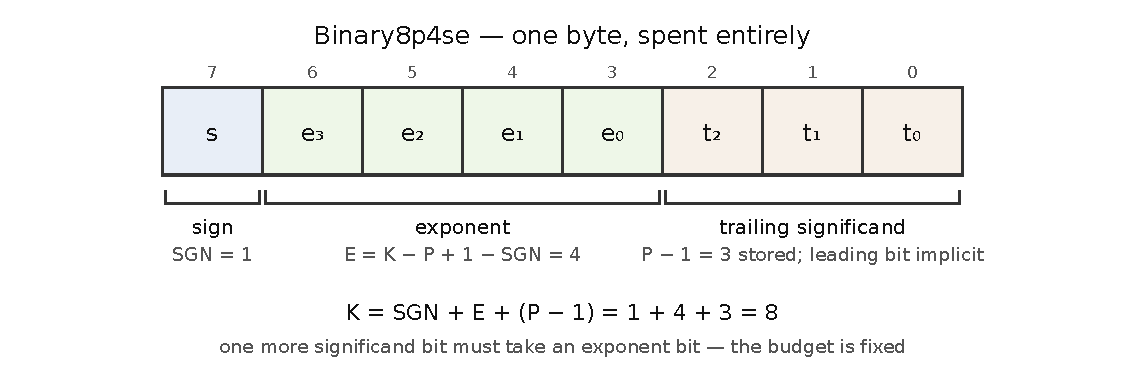
\includegraphics[max width=\linewidth]{assets/format_anatomy.pdf}
\caption{Bit-field anatomy of Binary8p4se: one sign bit, four exponent bits, three stored significand bits, with the leading significand bit implicit.}
\end{figure}




One sign bit if signed, \texttt{E = K − P + 1 − SGN} exponent bits, and \texttt{P − 1} stored significand bits. Raising precision by one bit removes one exponent bit; choosing a format is choosing this trade.



\texttt{using SmallFloats} exports the 120 aliases at \texttt{K ≤ 8}. The other 384 are available three ways — fully qualified, via \texttt{using SmallFloats.Formats}, or programmatically:




\nopagebreak[4]
\begin{minted}{jlcon}
julia> T = format(16, 6, true, true)
Binary16p6se

julia> codeunit_type(T), SmallFloats.datumcarrier(T)
(UInt16, Float64)
\end{minted}



Code points occupy a \texttt{UInt8} at \texttt{K ≤ 8} and a \texttt{UInt16} above. \texttt{decode} returns the format{\textquotesingle}s \emph{datum carrier}: \texttt{Float64} for the 432 formats it holds exactly, \texttt{Float128} or an exact dyadic carrier for the other 72. Both are representation details; the value model does not change with \texttt{K}.



One practical caution. The abstract type \texttt{Binary\{8,4,true,true\}} is a supertype of the concrete \texttt{Binary8p4se}, and it is not a valid array element type: \texttt{Vector} of the abstract format boxes every element and loses all of the performance machinery. Use the concrete alias, or \texttt{format(...)}, in element types.



\section{A format, listed in full}



\label{981248173416556099}{}


Small formats can be inspected completely. \texttt{Binary4p2se} has 16 code points, and this listing is the entire format:




\nopagebreak[4]
\begin{minted}{jlcon}
julia> decode.(sort(Binary4p2se.(0x00:0x0f)))
16-element Vector{Float64}:
 NaN
 -Inf
  -2.0
  -1.5
  -1.0
  -0.75
  -0.5
  -0.25
   0.0
   0.25
   0.5
   0.75
   1.0
   1.5
   2.0
  Inf
\end{minted}



The same table for any format, in storage order or total order, is a few lines. No projection is involved — \texttt{decode} is exact and policy-free, so the table depends on the format alone:




\nopagebreak[4]
\begin{minted}{julia}
function codetable(::Type{F}; by::Symbol = :code) where {F<:Binary}
    U = codeunit_type(F)                        # UInt8 at K ≤ 8, UInt16 above
    vals = [F(U(c)) for c in 0:(1 << bitwidth(F)) - 1]
    by === :value && sort!(vals)                # total order: NaN first
    [(code = codepoint(v), value = decode(v)) for v in vals]
end
\end{minted}



\texttt{codetable(Binary4p2se)} lists code \texttt{0x08} — the sign bit alone — as the single NaN, with negatives mirroring the positives above it; \texttt{codetable(\allowbreak{}Binary4p2se; by = :value)} reproduces the sorted listing above. The reverse table, value → code, does need a projection: \texttt{codepoint(\allowbreak{}Convert(\allowbreak{}F, ρ, x))}, one rounding per entry.



Three P3109 design decisions are visible here. There is exactly one NaN, with no payloads and no quiet/signalling distinction. There is no negative zero; \texttt{T(-0.0)} projects to the single zero. And NaN sorts first, below −Inf: the draft{\textquotesingle}s total order places it at the opposite end from \texttt{Float64} sorting, which gives sorting and searching deterministic behavior. Finite formats (suffix \texttt{f}) assign the two infinity code points to two additional finite datums.



\section{Construction projects}



\label{8317558927995832252}{}



\begin{minted}{jlcon}
julia> x = Binary8p4se(1.6)
Binary8p4se(1.625 ⇆ 0x45)
\end{minted}



The number 1.6 is not among the format{\textquotesingle}s values. Its nearest neighbors are 1.5, 1.625, and 1.75, spaced 0.125 apart in this binade, so construction rounds to the nearest datum and stores that datum{\textquotesingle}s code point. Constructors from a \texttt{Real} never throw for representable magnitudes; they round.



\texttt{decode} and \texttt{codepoint} read back the two halves:




\nopagebreak[4]
\begin{minted}{jlcon}
julia> decode(x), codepoint(x)
(1.625, 0x45)
\end{minted}



\texttt{decode} never rounds; it is a lookup from code point to datum. The asymmetry matters: reading is exact, writing projects.



\section{The code-point rule}



\label{13234262959082347228}{}


An \texttt{Unsigned} argument means code point. Every other \texttt{Real} argument means a value to project. The integer type{\textquotesingle}s signedness is the entire distinction:




\nopagebreak[4]
\begin{minted}{jlcon}
julia> Binary8p4se(0x02), Binary8p4se(2)
(Binary8p4se(0.001953125 ⇆ 0x02), Binary8p4se(2.0 ⇆ 0x48))
\end{minted}



The same digit, read two ways, differs by a factor of 1024 here — and neither call is an error, so a wrongly-typed integer produces a valid, different result rather than a failure. Use unsigned integers when you mean stored identity (a byte read from a file, a wire format). Use signed integers or any other \texttt{Real} when you mean a number. When intent must be explicit regardless of the argument{\textquotesingle}s type, \texttt{Convert(T, ρ, x)} always projects numerically.



The round-trip law holds in one direction: \texttt{T(codepoint(x)) === x} for every valid code point. The other direction fails by design — \texttt{decode(T(1.6))} returns 1.625, because construction already chose a datum, and nothing downstream can recover the original argument.



\section{Predicates, stepping, classification}



\label{16759329318099337913}{}


The standard numeric vocabulary applies to every format: \texttt{isnan}, \texttt{isinf}, \texttt{isfinite}, \texttt{iszero}, \texttt{signbit}, \texttt{issubnormal}, along with \texttt{zero}, \texttt{one}, \texttt{eps}, \texttt{typemin}, and \texttt{typemax}, all answering from the format{\textquotesingle}s own grid. Stepping moves to the adjacent code point, and \texttt{Class} reports the draft{\textquotesingle}s classification:




\nopagebreak[4]
\begin{minted}{jlcon}
julia> NextGreaterThan(Binary8p4se(1.0))
Binary8p4se(1.125 ⇆ 0x41)

julia> Class(Binary8p4se(0.01))
ClassPosNormal::FPClass = 0x06
\end{minted}



\texttt{NextGreaterThan} and \texttt{NextLessThan} are the draft{\textquotesingle}s Next operations; \texttt{nextfloat} and \texttt{prevfloat} alias them.



One related distinction: Base{\textquotesingle}s lowercase \texttt{convert} is value-preserving on \texttt{Unsigned} input — \texttt{convert(\allowbreak{}Binary8p4se, 0x02)} is the value 2.0, not code point 2 — because Julia{\textquotesingle}s promotion machinery, \texttt{similar}, and \texttt{fill} depend on that behavior. The code-point reading belongs to the constructor alone. Prefer \texttt{T(x)} or \texttt{Convert(T, ρ, x)} in your own code and leave bare \texttt{convert} to the places Base itself calls it.



\section{Display}



\label{12429740135947470305}{}


Four styles render the same value: \texttt{:value} (\texttt{1.625}), \texttt{:codepoint} (\texttt{0x45}), \texttt{:datum} (\texttt{1.625 ⇆ 0x45}), and \texttt{:typed} (\texttt{Binary8p4se(\allowbreak{}1.625 ⇆ 0x45)}). Select one process-wide with \texttt{set\_\allowbreak{}show\_\allowbreak{}style!} or per-stream with the \texttt{:binary\_\allowbreak{}show\_\allowbreak{}style} \texttt{IOContext} property. Display is presentation only; no kernel or comparison reads it. This guide uses \texttt{:typed} throughout.



\section{Next}



\label{9862256287407127426}{}


Values exist but nothing has computed with them. Construction from a \texttt{Real} rounded, and this chapter did not say by what rule. The rule is a policy the caller selects, and it is the subject of \href{computing.md}{Computing}.





\chapter{Computing}



\label{6001489924641501409}{}


Every numeric operation follows the same three steps: decode the operands, compute the mathematically exact result over the extended reals, and project once. There is no arithmetic {\textquotedbl}in the format{\textquotedbl} and no accumulated rounding inside an operation. Rounding error arises only at the single point where the exact result becomes a code point. This chapter covers that point: the two policy choices that decide it, and how to keep the decision stable.



\section{One projection, named in the call}



\label{13836310120754226451}{}



\begin{minted}{jlcon}
julia> x, y = Binary8p4se(1.6), Binary8p4se(0x46);

julia> Add(Binary8p4se, RNE_SN, x, y)
Binary8p4se(3.5 ⇆ 0x4e)
\end{minted}



The call reads left to right: operation, result format, projection specification, operands. The exact sum, 1.625 + 1.75 = 3.375, is not a datum; it lies exactly halfway between 3.25 and 3.5, so the stored result is determined entirely by policy. \texttt{RNE\_\allowbreak{}SN} rounds to nearest with ties to even, selecting 3.5, then applies the draft{\textquotesingle}s \texttt{SatNone} boundary rules. A different projection could land the same sum on 3.25. The projection therefore appears in the argument list: it is part of the operation, not an ambient setting.



The ordinary Julia spelling uses the current session default:




\nopagebreak[4]
\begin{minted}{jlcon}
julia> x + y
Binary8p4se(3.5 ⇆ 0x4e)
\end{minted}



Use \texttt{+} and the other operators for interactive work. Use \texttt{Add(T, ρ, ...)} in code whose results must not depend on session state.



\section{Rounding and saturation}



\label{4169779663468363235}{}


A \texttt{ProjSpec} pairs two independent choices. Rounding selects the neighbor: six deterministic modes (nearest-ties-even, nearest-ties-away, toward positive, toward negative, toward zero, to-odd), with every pairing predefined under names such as \texttt{RNE\_\allowbreak{}SN} and \texttt{RTZ\_\allowbreak{}SF}. Saturation decides what an out-of-range result becomes: \texttt{SatFinite} clamps to the finite extremes, \texttt{SatPropagate} preserves representable infinities, and \texttt{SatNone} applies the draft{\textquotesingle}s full domain-, sign-, and direction-dependent rows. \texttt{SatNone} does not mean {\textquotedbl}no saturation{\textquotedbl}; it means neither simplifying policy was selected.



The axes separate cleanly on one overflow. Note first that \texttt{Binary8p4se(200.0)} already projected during construction — 200 ties between 192 and 208 and lands on 192 — so both multiplies below compute the exact product 384, which exceeds the largest finite datum, 224:




\nopagebreak[4]
\begin{minted}{jlcon}
julia> w, two = Binary8p4se(200.0), Binary8p4se(2.0);

julia> Multiply(Binary8p4se, RNE_SN, w, two)   # nearest + draft rows → Inf
Binary8p4se(Inf ⇆ 0x7f)

julia> Multiply(Binary8p4se, RNE_SF, w, two)   # nearest + clamp → 224
Binary8p4se(224.0 ⇆ 0x7e)

julia> Multiply(Binary8p4se, RTZ_SN, w, two)   # toward zero + draft rows → 224
Binary8p4se(224.0 ⇆ 0x7e)
\end{minted}



The first two calls differ in saturation; the first and third differ in rounding. The third is the subtle case: rounding runs first and knows nothing about range, and saturation then classifies the out-of-range result with the rounding mode passed in — so a directed mode pointing away from the overflow yields the finite extreme even under \texttt{SatNone}. Choose \texttt{SatNone} when an overflow should remain observable as an infinity, \texttt{SatFinite} when downstream code cannot absorb one.



\section{Stochastic rounding}



\label{5064376698567748197}{}


The three stochastic families (\texttt{StochasticA/B/C}, with random-bit budget \texttt{N}) make the landing depend on the exact fractional position and a draw \texttt{R ∈ 0:2{\textasciicircum}N−1}. The distribution is part of the definition: projecting 2 + 3/64 under \texttt{RSA\_\allowbreak{}SN(4)}, a value three sixteenths of the way from 2.0 to 2.25, rounds upward for exactly 3 of the 16 possible draws. Fixing \texttt{R} makes a single projection exactly reproducible, which suits tests:




\nopagebreak[4]
\begin{minted}{jlcon}
julia> σ = RSA_SN();                 # StochasticA, default N = 8

julia> a, b = Binary8p4se(2.0), Binary8p4se(0.03125);

julia> Add(Binary8p4se, σ, a, b; R = 0)
Binary8p4se(2.0 ⇆ 0x48)      # smallest draw: rounds down

julia> Add(Binary8p4se, σ, a, b; R = 255)
Binary8p4se(2.25 ⇆ 0x49)     # largest draw: rounds up
\end{minted}



For streams, pass a seeded \texttt{rng}; stochastic projection draws from the same generator as any value draws, so one seed reproduces a whole pipeline. An out-of-range \texttt{R} is an error, not a silently wrapped value.



\section{Random values}



\label{13027969696381432085}{}


\texttt{rand} and \texttt{randn} work for every format, and both accept an explicit RNG for reproducibility:




\nopagebreak[4]
\begin{minted}{jlcon}
julia> rand(Xoshiro(1), Binary8p4se)
Binary8p4se(0.0703125 ⇆ 0x21)

julia> rand(Xoshiro(8), Binary8p4se, 4)
4-element Vector{Binary8p4se}:
 Binary8p4se(0.40625 ⇆ 0x35)
 Binary8p4se(0.021484375 ⇆ 0x13)
 Binary8p4se(0.75 ⇆ 0x3c)
 Binary8p4se(0.28125 ⇆ 0x31)
\end{minted}



Scalar \texttt{rand} takes a \texttt{projection} keyword. The default is a floor projection, which keeps results in \texttt{[0, 1)} as \texttt{rand}{\textquotesingle}s contract requires; opting into \texttt{RTP\_\allowbreak{}SN} or \texttt{RNE\_\allowbreak{}SN} can return exactly 1.0, since mass near the top rounds up. The array and in-place forms always use the defaults — for an array under another projection, draw scalars explicitly.



\section{Session defaults}



\label{3970345369238056532}{}


Five process-wide defaults back the convenience forms: \texttt{DefaultType}, \texttt{DefaultReturnType}, \texttt{DefaultRoundingMode}, \texttt{DefaultSaturationMode}, and \texttt{DefaultProjection}. The projection default and its two components remain coherent regardless of which setter ran last:




\nopagebreak[4]
\begin{minted}{julia}
DefaultProjection() === ProjSpec(DefaultRoundingMode(), DefaultSaturationMode())
\end{minted}



A setter mutates state shared by every module in the process, and nothing scopes or restores it:




\nopagebreak[4]
\begin{minted}{jlcon}
julia> w * two                            # follows the default: RNE_SN → Inf
Binary8p4se(Inf ⇆ 0x7f)

julia> DefaultProjection!(RTZ_SF);

julia> w * two                            # every convenience call changed
Binary8p4se(224.0 ⇆ 0x7e)

julia> DefaultProjection!(RNE_SN)         # restore; the setting is process-wide
(NearestTiesToEven, SatNone)

julia> Multiply(Binary8p4se, RNE_SN, w, two)   # explicit ρ never reads a default
Binary8p4se(Inf ⇆ 0x7f)
\end{minted}



Library code and experiments should name \texttt{T} and \texttt{ρ} explicitly. The setters are appropriate for interactive sessions you control.



\section{Interaction with Julia{\textquotesingle}s numeric model}



\label{12536725406993873247}{}


Same-format expressions use ordinary Julia spellings — \texttt{+ - * /}, \texttt{exp}, \texttt{sqrt}, comparisons — each equivalent to one draft operation under the session default. Three boundaries are deliberate:



\begin{itemize}
\item \textbf{Mixed \texttt{Binary} formats do not promote.} No automatic rule can soundly pick a containing format (most format pairs have none within the grid, and pairwise selection is not associative), so cross-format arithmetic requires an explicit \texttt{Convert}.


\item \textbf{\texttt{Binary} with an ordinary number promotes to the format{\textquotesingle}s carrier.} \texttt{Binary8p4se(1.5) + 2.0} returns the \texttt{Float64} value \texttt{3.5}, not a \texttt{Binary} value; the 72 wide formats promote to \texttt{BigFloat} instead, since a \texttt{Float64} cannot hold their datums. Project back explicitly when the result should be in the format.


\item \textbf{Some inputs are refused rather than double-rounded.} \texttt{Convert} accepts every type it can project exactly: \texttt{Binary} values, machine floats, \texttt{Float128}, integers, \texttt{BigFloat}. A \texttt{Rational} would require a hidden second rounding to reach a carrier, so it throws with guidance — convert to a supported carrier first, making that rounding your explicit choice.

\end{itemize}


Two draft semantics differ from IEEE 754 by design. \texttt{Divide(x, 0)} is NaN for every \texttt{x}, including ±Inf, and \texttt{Recip(±Inf)} is 0 — there are no signed-infinity quotients. And the total order places the single NaN first, below −Inf, so sorting a \texttt{Binary} vector leads with NaN.



\section{Next}



\label{9862256287407127426-dup1}{}


This chapter computed one value at a time. The same contract must hold for large arrays, fused reductions, and storage at true bit width, without acceleration changing any code point. That is the subject of \href{data.md}{Data at Scale}.





\chapter{Data at Scale}



\label{15729904777561585153}{}


One rule governs this chapter: acceleration may change how work is scheduled, never which code point is returned. Arrays, cached tables, fused block reductions, and packed storage are four schedules for the same exact-then-project computation.



\section{Arrays and tables}



\label{4990902378038015438}{}


Every operation has array methods with the scalar argument shape, operands replaced by arrays. Each element is exactly the scalar answer:




\nopagebreak[4]
\begin{minted}{jlcon}
julia> A = Binary8p4se.([-1.0, 0.5, 2.0]);

julia> Exp(Binary8p4se, RNE_SN, A)
3-element Vector{Binary8p4se}:
 Binary8p4se(0.375 ⇆ 0x34)
 Binary8p4se(1.625 ⇆ 0x45)
 Binary8p4se(7.5 ⇆ 0x57)
\end{minted}



Under a deterministic projection, a unary or binary operation is a finite function on code points, so the package may cache it. The first array call for a signature can build a result table; later calls gather from it. Every table entry is produced by the scalar path and compared against it by the test gates, so declining the table — stochastic specs draw per element, and large signatures exceed the byte budget — means running the same scalar path per element, never computing a different answer. \texttt{table\_\allowbreak{}policy} reports which shape a signature receives and why. When benchmarking, measure the first (table-building) call separately from warm calls.



Sorting uses integer order keys and, for large vectors, an O(n) counting sort. Order follows the draft{\textquotesingle}s total order, with the single NaN first.



\section{Choosing a format}



\label{10423729552281943573}{}


Format choice is a measurement, not a guess. At fixed bitwidth, precision trades against range, and the trade should be evaluated on data shaped like yours. For a unit-scale Gaussian sample of 50 000 values projected through each 8-bit signed extended format under \texttt{RNE\_\allowbreak{}SF}:




\nopagebreak[4]
\begin{minted}{text}
Binary8p5se  rmse = 0.0133   maxfinite = 15.0
Binary8p4se  rmse = 0.0266   maxfinite = 224.0
Binary8p3se  rmse = 0.0528   maxfinite = 49152.0
Binary8p2se  rmse = 0.103    maxfinite = 2.147483648e9
\end{minted}



RMSE roughly doubles for each significand bit given up, while the finite range grows enormously. For this sample no format overflows, so the extra range is unused and the highest precision wins. On wider-spread data the comparison changes, which is why three numbers should accompany any quantization choice: aggregate error (RMSE), worst single error, and the overflow or clamp rate. A format can score well on the first and fail on either of the others. When the dynamic range genuinely exceeds what the precision budget allows, do not buy range with a wider element format — get it from a block scale, below.



Unsigned formats suit quantities that are never negative (probabilities, memberships, normalized scores); finite formats suit domains where an infinity would be meaningless. Both spend otherwise-idle code points on resolution.



The decision, as a checklist:



\begin{itemize}
\item[1. ] Never negative? Use an unsigned format (\texttt{u}).


\item[2. ] Is an infinity a meaningful outcome? If not, use a finite format (\texttt{f}).


\item[3. ] Run the three-number report (RMSE, worst error, overflow rate) on data shaped like yours; take the highest precision whose overflow rate is acceptable.


\item[4. ] Range still exceeds the precision budget? Use a block scale, below — not a wider element format.


\item[5. ] Storage- or bandwidth-bound? Pack, at the end (packing changes layout, not the quantization).

\end{itemize}


\section{Blocks}



\label{13626648213057379036}{}


When data spans more range than a narrow element format holds, widening the element spends bits on exponent that were wanted for precision. A \texttt{Block\{B,FS,FE\}} shares one scale (format \texttt{FS}) across \texttt{B} elements (format \texttt{FE}); each lane represents \texttt{scale × element}. This is the draft{\textquotesingle}s MX-style scheme. Construct a block directly, or quantize a tuple and let the draft{\textquotesingle}s algorithm derive the scale from the largest finite magnitude:




\nopagebreak[4]
\begin{minted}{jlcon}
julia> Block(Binary8p1uf(4.0), Binary8p4se(1.5), Binary8p4se(-0.75),
             Binary8p4se(2.0), Binary8p4se(0.5))
Block{4, Binary8p1uf, Binary8p4se}(Binary8p1uf(4.0 ⇆ 0x82), (…))

julia> ConvertToBlockMaxAbsFinite(Binary8p1uf, Binary8p4se, RNE_SN, RNE_SN,
           (Binary8p4se(100.0), Binary8p4se(-12.0), Binary8p4se(0.5), Binary8p4se(3.0)))
Block{4, Binary8p1uf, Binary8p4se}(Binary8p1uf(64.0 ⇆ 0x86), (…))
\end{minted}



The arguments read in order: scale format, element format, a projection for the scale, a projection for the elements, then the values. Here the algorithm chose scale 64 from the largest element, 100, and projected each element against it. \texttt{ConvertFromBlock(\allowbreak{}T, ρ, b)} reads a block back out as plain values, decoding each \texttt{scale × element} exactly and projecting once. Scale formats are conventionally unsigned with precision 1 (\texttt{Binary8p1uf}): every datum is a power of two, so dividing by the scale is exact.



Block reductions are where the exactness contract does real work. A reduction decodes every lane exactly, accumulates exactly — an integer span filter proves a \texttt{Float128} accumulator suffices, or an arbitrary-precision accumulator sized from the formats takes over — and projects once:




\nopagebreak[4]
\begin{minted}{jlcon}
julia> b = Block(Binary8p1uf(0.5), (Binary8p4se(80.0), Binary8p4se(-0.375),
                                    Binary8p4se(-5.5), Binary8p4se(2.25)));

julia> SmallFloats.blockdecode(b)              # the exact lane values
(40.0, -0.1875, -2.75, 1.125)

julia> BlockReduceAdd(Binary8p4se, RNE_SN, b)  # exact sum 38.1875, projected once
Binary8p4se(40.0 ⇆ 0x6a)

julia> lanes = SmallFloats.blockdecode(b);

julia> foldl((a, v) -> Add(Binary8p4se, RNE_SN, a, Convert(Binary8p4se, RNE_SN, v)),
             lanes; init = zero(Binary8p4se))  # rounding at every step
Binary8p4se(36.0 ⇆ 0x69)
\end{minted}



The exact sum is 38.1875 and the correct projection is 40. Lane-by-lane accumulation lands on 36 — a defined-result error that grows with \texttt{B}. \texttt{BlockDotProduct} gives the same guarantee for fused products: on random 32-lane blocks, the entire difference from the \texttt{Float64} dot product is the initial quantization of the inputs; accumulation contributes nothing.



One pitfall dominates block practice. \texttt{ConvertToBlockMaxAbsFinite} quantizes a tuple, deriving the scale from the largest finite magnitude — but it takes elements that are already \texttt{Binary}. If raw data is staged through the narrow element format first, \texttt{SatFinite} clamps the large values before the block scale can absorb them, and blocking gains nothing. Measured on a 64×64 matrix whose rows span roughly 2{\textasciicircum}16 in scale: direct \texttt{Binary8p4se} conversion has relative error 0.616, element-format staging 0.617, and staging through the wide-range \texttt{Binary8p2se} before block-quantizing 0.109 — the staging format{\textquotesingle}s own precision. Stage wide, then block-quantize. At \texttt{B = 32} with an 8-bit scale, storage costs 8.25 bits per value.



\section{Packed storage}



\label{8567984038512272605}{}


A \texttt{Vector\{Binary5p2se\}} spends a full byte on each 5-bit code point. \texttt{PackedVector(v)} stores elements at true bit width. It is a complete \texttt{AbstractVector\{F\}} — indexing, iteration, \texttt{collect} — and \texttt{vmap} computes on it directly, unpacking tiles internally:




\nopagebreak[4]
\begin{minted}{jlcon}
julia> n = 1_000_000;

julia> model = [Binary5p2se(UInt8(rand(0:31))) for _ in 1:n];

julia> pv = PackedVector(model);

julia> (sizeof(model), sizeof(pv.data))
(1000000, 625000)
\end{minted}



The rule is store packed, compute unpacked; there is deliberately no in-place packed arithmetic. Packing pays when memory or bandwidth is the constraint — for example, a large quantized model held resident. For compute-only work an ordinary \texttt{Vector\{F\}} avoids the unpack cost.



\section{Float16 and BFloat16}



\label{10938659776745642755}{}


\texttt{Binary16p11se} resembles \texttt{Float16}, and \texttt{Binary16p8se} resembles \texttt{BFloat16}, but P3109{\textquotesingle}s exponent bias differs from IEEE{\textquotesingle}s by one (16 versus 15; 128 versus 127). Every code point therefore denotes a value a factor of two away from its IEEE counterpart; largest finite values are 65472 versus 65504, there is one NaN rather than 2046 encodings, and no negative zero.




\begin{minted}{jlcon}
julia> using SmallFloats.Formats

julia> Convert(Binary16p11se, RNE_SF, Float16(1.5))    # a conversion: 1.5 ↦ 1.5
Binary16p11se(1.5 ⇆ 0x4200)

julia> reinterpret(Binary16p11se, Float16(1.5))        # the same bits: 1.5 ↦ 0.75
Binary16p11se(0.75 ⇆ 0x3e00)
\end{minted}



The reinterpreted value is wrong by a factor of two, with no error and no warning — the most dangerous operation in cross-format work, because the numbers look plausible. Use \texttt{Convert} across the IEEE boundary, never \texttt{reinterpret}. \texttt{datumsexact} reports which format pairs round-trip losslessly.



\section{Next}



\label{9862256287407127426-dup2}{}


\href{worked\_\allowbreak{}example.md}{A Worked Example} composes this chapter and the two before it into one measured quantization task, end to end.





\chapter{A Worked Example}



\label{15995443143905973460}{}


The preceding chapters in one task: choose a format for real data, quantize, measure what the choice cost, and record what produced the numbers. The pattern transfers directly to model weights, activations, or any signal.



\section{The data, and an explicit policy}



\label{11636787435248503912}{}


A fixed seed makes the session reproducible; \texttt{RNE\_\allowbreak{}SF} — nearest, ties to even, clamp to finite — is named once and used throughout, so the report stays meaningful even if a session default changes elsewhere:




\nopagebreak[4]
\begin{minted}{julia}
using SmallFloats, Random, Statistics

rng = Xoshiro(42)
w = randn(rng, 50_000) .* 0.25        # a typical trained-weight scale
\end{minted}



\section{Measure, with three numbers}



\label{3943201719433937344}{}


One number is not enough evidence for a quantization choice. Aggregate error can look fine while single values are badly wrong, and both can look fine while the tails overflow. Report all three:




\nopagebreak[4]
\begin{minipage}{\linewidth}
\begin{minted}{julia}
function quantization_report(::Type{F}, x; projection = RNE_SF) where {F}
    q = [Convert(F, projection, xi) for xi in x]
    y = decode.(q)
    finite = isfinite.(y)
    (
        format = formatname(F),
        rmse = sqrt(mean((x[finite] .- y[finite]).^2)),
        max_error = maximum(abs.(x[finite] .- y[finite])),
        nonfinite_rate = count(!isfinite, y) / length(y),
        boundary_rate = count(v -> abs(v) == decode(MaxFiniteOf(F)), y) / length(y),
    )
end

quantization_report(Binary8p4se, w)
\end{minted}




\begin{minted}{text}
(format = :Binary8p4se, rmse = 0.0066, max_error = 0.0622,
 nonfinite_rate = 0.0, boundary_rate = 0.0)
\end{minted}
\end{minipage}




Average damage is small, the worst single value is off by ten times the average, and nothing overflowed — for this sample, range was never the binding constraint.



\section{Compare candidates under one policy}



\label{4920482121782597622}{}


Same sample, same projection, four formats — never change the data and the policy in the same experiment:




\nopagebreak[4]
\begin{minipage}{\linewidth}
\begin{minted}{julia}
for F in (Binary8p5se, Binary8p4se, Binary8p3se, Binary8p2se)
    r = quantization_report(F, w)
    println(rpad(String(r.format), 12), " rmse=", round(r.rmse; sigdigits=3),
            "  max=", round(r.max_error; sigdigits=3),
            "  nonfinite=", r.nonfinite_rate, "  boundary=", r.boundary_rate)
end
\end{minted}




\begin{minted}{text}
Binary8p5se  rmse=0.00356  max=0.0256  nonfinite=0.0  boundary=0.0
Binary8p4se  rmse=0.00662  max=0.0622  nonfinite=0.0  boundary=0.0
Binary8p3se  rmse=0.0132   max=0.0881  nonfinite=0.0  boundary=0.0
Binary8p2se  rmse=0.0261   max=0.162   nonfinite=0.0  boundary=0.0
\end{minted}
\end{minipage}




RMSE roughly doubles per significand bit given up, exactly as the datum spacing does. Every format holds this data without overflow, so the range the lower-precision formats offer goes unused and \texttt{Binary8p5se} wins outright. On wider-spread data the last two columns stop reading zero and the ranking changes — which is what they are there to catch.



\section{Inspect the worst misses}



\label{18179706212253785775}{}



\begin{minipage}{\linewidth}
\begin{minted}{julia}
q = [Convert(Binary8p4se, RNE_SF, x) for x in w]
err = abs.(w .- decode.(q))
worst = partialsortperm(err, 1:3; rev = true)
[(w[i], decode(q[i]), err[i]) for i in worst]
\end{minted}




\begin{minted}{text}
(-1.06279, -1.125, 0.06221)
(-1.06092, -1.0,   0.06092)
(-1.06967, -1.125, 0.05533)
\end{minted}
\end{minipage}




The worst errors cluster just past 1.0, where \texttt{Binary8p4se}{\textquotesingle}s spacing widens to 0.125 at the binade boundary — a structural property of the format, not an unlucky sample. Knowing where the errors live says whether a different format would help or the data needs rescaling. If failures cluster by row or channel scale instead, use a block scale (see \href{data.md}{Data at Scale}).



\section{Record what produced the result}



\label{12845234384692473716}{}



\begin{minted}{julia}
d = conformance_dict()          # formats, operations, specializations, approximations
rev = draft_revision()          # "IEEE P3109/D1, uploaded 2026-07-17"
\end{minted}



Serialize \texttt{d} with any JSON or TOML writer and store it, the draft revision, the chosen format, the projection name, and the seed beside the quantized artifact. A later reader can then reproduce the numbers or explain a difference without guessing what the session looked like.



\section{Next}



\label{9862256287407127426-dup3}{}


\href{assurance.md}{Assurance} covers the record-keeping used above in full: the provenance test, measured approximation, and how the defined path itself is verified.





\chapter{Assurance}



\label{14478627307656753823}{}


When two runs disagree, exactly three causes are legitimate: the policy changed, the policy itself requests randomness, or a registered approximation was selected. Anything else is a defect. This chapter provides the tools that make that determination and the records that support it: the provenance test, the measured-approximation registry, the exportable conformance declaration, and a summary of how the defined path is verified.



\section{The provenance test}



\label{17718339924439357099}{}


When two runs differ, check in order:



\begin{itemize}
\item[1. ] Did the operation, result format, or projection specification change?


\item[2. ] Is the projection stochastic, and did the draw or RNG stream change?


\item[3. ] Did the call explicitly select a registered approximation?


\item[4. ] Did process-global defaults change between calls?

\end{itemize}


If all four answers are no, a changed code point is a defect and should be reported as one. For experiments that must be reproducible, record the result format, the projection specification, the RNG algorithm and seed, and any approximation{\textquotesingle}s name and measured bound alongside the results.



\section{Measured approximation}



\label{2780525639147152128}{}


The default API never substitutes an approximation. A faster, inexact kernel enters only through the registry, and the registry measures its worst-case deviation — in code points along the total order, exhaustively where the input space permits — rather than accepting a declared figure:




\nopagebreak[4]
\begin{minted}{jlcon}
julia> one4 = Binary8p4se(1.0);

julia> hardtanh(x) = Clamp(Binary8p4se, RNE_SN, x, Negate(one4), one4);

julia> κ, exhaustive = measure_kappa(hardtanh, :Tanh, Binary8p4se,
                                     (Binary8p4se,), RNE_SN)
(4.0, true)                # worst deviation: 4 code points, all 256 inputs checked
\end{minted}



A declaration that understates the measurement is rejected, and no partial registration state remains:




\nopagebreak[4]
\begin{minted}{jlcon}
julia> register_approx!(:hardtanh_act, :Tanh, Binary8p4se,
                        (Binary8p4se,), RNE_SN, hardtanh; κ=1)
ERROR: ArgumentError: declared κ = 1.0 understates measured κ = 4.0 — registration rejected
\end{minted}



Registered with a truthful bound, the implementation is retrieved by name (\texttt{approx}, \texttt{list\_\allowbreak{}approx}), its κ is queryable, and it appears in the conformance declaration automatically. Code-point bounds also support decision rules: two defined results more than 2κ apart cannot have their comparison inverted by the approximate evaluator, which makes pruning with a cheap evaluator provably sound.



\section{The conformance declaration}



\label{15718388096894276699}{}


\texttt{conformance()} returns a live statement of the session: formats, operations, mode vocabulary, the table specializations built so far, and every registered approximation. \texttt{conformance\_\allowbreak{}dict()} is the plain-\texttt{Dict} form for JSON or TOML export:




\nopagebreak[4]
\begin{minipage}{\linewidth}
\begin{minted}{julia}
d = conformance_dict()
(d["package"], length(d["formats"]), length(d["operations"]),
 [s["op"] for s in d["cached_specializations"]])
\end{minted}




\begin{minted}{text}
("SmallFloats.jl 0.4.0", 504, 52, Any[])
\end{minted}
\end{minipage}




The first three entries are package properties: 504 formats, 52 operations, always. The fourth is session-dependent — empty here because this session had made no array call yet — so snapshot the declaration after the work, not at the top of a script. \texttt{draft\_\allowbreak{}revision()} reports the implemented draft revision (\texttt{IEEE P3109/\allowbreak{}D1, uploaded 2026-07-17}); include it with any exported artifact.



\section{Verifying your own code}



\label{12572045495842974798}{}


The same exhaustive method is available to application code, because format input spaces are small enough to enumerate. A stochastic-rounding distribution, for example, is checkable exactly rather than statistically: the value 2 + 3/64 sits at fraction 3/16 of an ulp, so \texttt{StochasticA\{4\}} must round it up for exactly 3 of the 16 draws —




\begin{minipage}{\linewidth}
\begin{minted}{julia}
σ4 = RSA_SN(4)
x = 2.0 + 3/64
count(decode(SmallFloats.project(Binary8p4se, σ4, x; R)) == 2.25 for R in 0:15)
\end{minted}




\begin{minted}{text}
3
\end{minted}
\end{minipage}




Sweeping \texttt{R} turns a statistical question about bias into an exhaustive one.



Ordering guarantees are checkable the same way. Ranking and decision systems consume scores through order, so a conversion between formats must be monotone — and with a few hundred datums per format, that is provable by walking every value in total order and confirming its image never goes backward:




\nopagebreak[4]
\begin{minipage}{\linewidth}
\begin{minted}{julia}
using SmallFloats: order_key

function monotone_conversion(::Type{From}, ::Type{To}) where {From,To}
    prev = nothing
    for v in sort(From.(0x00:UInt8(2^bitwidth(From) - 1)))
        isnan(decode(v)) && continue
        g = Convert(To, RNE_SN, v)
        prev !== nothing && order_key(g) < order_key(prev) && return false
        prev = g
    end
    true
end
monotone_conversion(Binary8p3se, Binary8p4se)
\end{minted}




\begin{minted}{text}
true
\end{minted}
\end{minipage}




A ranking pipeline whose conversions all pass this audit cannot invert a preference by changing formats. The same pattern — enumerate the inputs, compare against an independently computed reference — verifies quantizers and custom fused kernels; the full manual{\textquotesingle}s Verify Custom Code page gives worked recipes.



\section{How the defined path is verified}



\label{6804462531286882542}{}


The test suite enumerates rather than samples wherever the input space allows, and reports {\textquotedbl}sampled{\textquotedbl} explicitly where it does not. Because formats are finite, most correctness claims are checked by exhaustion: every code point of every format round-trips; cached tables compare entry-for-entry with the scalar path; the optimized rounding core compares against the generic one; and two independent high-precision references (\texttt{Float128}-first and pure-MPFR builds) must agree bit-for-bit. Disabling the \texttt{Float128} machinery (\texttt{ENV[{\textquotedbl}SmallFloats\_\allowbreak{}Float128{\textquotedbl}] = {\textquotedbl}disable{\textquotedbl}}) is itself a tested equivalence: identical results, different speed.



Structurally, there is one write path. Every code point the package produces passes through \texttt{RoundToPrecision → Saturate → Encode}, fed by exact arithmetic on a carrier the format selects — \texttt{Float64} where exact, \texttt{Float128} above it, an exact dyadic carrier for the widest formats, with MPFR enclosures deciding the remainder. No second rounding routine exists, and nothing approximate is reachable outside the registry. The full manual{\textquotesingle}s Technical Guide covers the architecture, the oracle{\textquotesingle}s rigor classes, and the verification gates in detail.



\section{Next}



\label{9862256287407127426-dup4}{}


\href{reference.md}{Quick Reference} collects the names and signatures from all four chapters in brief.





\chapter{Quick Reference}



\label{10518953264959401364}{}


Names and signatures in brief. For semantics, see the preceding chapters; for exhaustive tables, the full manual{\textquotesingle}s Reference section.



\section{Values in and out}



\label{6161161780416834527}{}



\begin{minted}{julia}
Binary8p4se(1.6)          # Real → project to nearest datum
Binary8p4se(0x45)         # Unsigned → CODE POINT (validated)
Convert(T, ρ, x)          # explicit projection, numeric for every integer
decode(x)                 # the exact datum, on the format's carrier
codepoint(x)              # the stored identity
T(codepoint(x)) === x     # the round-trip law
\end{minted}



\section{Format queries}



\label{11700971017834573131}{}


Pure functions of the type parameters; each takes a type or a value, and folds to a constant either way.




\begin{minted}{julia}
bitwidth(T)  precision(T)  issigned(T)  isextended(T)
expbias(T)   expbitwidth(T)  trailingsigbits(T)
MaxFiniteOf(T)  MinFiniteOf(T)  MinPositiveOf(T)
MinNormalOf(T)  MaxSubnormalOf(T)
format(K, P, SGN, EXT)    # programmatic route to any of the 504
\end{minted}



Draft-named twins exist throughout: \texttt{BitwidthOf}, \texttt{PrecisionOf}, \texttt{ExponentBiasOf}, ….



\needspace{26\baselineskip}
\section{Projection specifications}



\label{714366806163910976}{}


\texttt{ProjSpec(\allowbreak{}rounding, saturation)}; every deterministic pairing is predefined as \texttt{R<mode>\_\allowbreak{}S<mode>}:




\begin{table}[h]
\centering
\begin{tabulary}{\linewidth}{L L L L}
\toprule
 & \texttt{SatNone} & \texttt{SatFinite} & \texttt{SatPropagate} \\
\toprule
\texttt{NearestTiesToEven} & \texttt{RNE\_\allowbreak{}SN} & \texttt{RNE\_\allowbreak{}SF} & \texttt{RNE\_\allowbreak{}SP} \\
\texttt{NearestTiesToAway} & \texttt{RNA\_\allowbreak{}SN} & \texttt{RNA\_\allowbreak{}SF} & \texttt{RNA\_\allowbreak{}SP} \\
\texttt{TowardPositive} & \texttt{RTP\_\allowbreak{}SN} & \texttt{RTP\_\allowbreak{}SF} & \texttt{RTP\_\allowbreak{}SP} \\
\texttt{TowardNegative} & \texttt{RTN\_\allowbreak{}SN} & \texttt{RTN\_\allowbreak{}SF} & \texttt{RTN\_\allowbreak{}SP} \\
\texttt{TowardZero} & \texttt{RTZ\_\allowbreak{}SN} & \texttt{RTZ\_\allowbreak{}SF} & \texttt{RTZ\_\allowbreak{}SP} \\
\texttt{ToOdd} & \texttt{RTO\_\allowbreak{}SN} & \texttt{RTO\_\allowbreak{}SF} & \texttt{RTO\_\allowbreak{}SP} \\
\bottomrule
\end{tabulary}

\end{table}



Stochastic constructors: \texttt{RSA\_\allowbreak{}SN(N)}, \texttt{RSB\_\allowbreak{}SF(N)}, \texttt{RSC\_\allowbreak{}SP(N)}, … — families A/B/C crossed with the saturation modes, \texttt{N} random bits (default 8). Pass \texttt{rng} for a stream or \texttt{R ∈ 0:2{\textasciicircum}N−1} for one exact draw. \texttt{RNE\_\allowbreak{}SN} is the initial session default.



\section{Operations}



\label{4250268531802119509}{}


52 draft operations — 30 unary, 18 binary, 3 ternary, plus \texttt{Convert} — every one spelled \texttt{Op(fr, ρ, operands…)} with a same-format convenience \texttt{Op(x…)}, array methods, and \texttt{Block}/\allowbreak\texttt{Scaled} variants. Families: sign and arithmetic (\texttt{Abs} … \texttt{Divide}, fused \texttt{FMA}/\allowbreak\texttt{FAA}), roots and exp/log, trig, hyperbolic, π-scaled trig, \texttt{Softplus}/\allowbreak\texttt{Hypot}/\texttt{ArcTan2}, extrema and \texttt{Clamp}, comparisons and \texttt{TotalOrder}, format queries, \texttt{NextGreaterThan} / \texttt{NextLessThan}. Base spellings (\texttt{+}, \texttt{exp}, \texttt{sqrt}, \texttt{min}, \texttt{nextfloat}, …) map one-to-one onto same-format calls under the session default.



\section{Session defaults}



\label{3970345369238056532-dup1}{}


Read with \texttt{DefaultX()}, set with \texttt{DefaultX!(v)}:




\nopagebreak[4]
\begin{minted}{julia}
DefaultType        DefaultReturnType
DefaultRoundingMode  DefaultSaturationMode  DefaultProjection
\end{minted}



The projection default and its two component defaults stay coherent no matter which setter ran last. All five are process-global; name \texttt{T} and \texttt{ρ} explicitly in anything that must be reproducible.



\section{Display}



\label{12429740135947470305-dup1}{}


\texttt{set\_\allowbreak{}show\_\allowbreak{}style!(s)} / \texttt{get\_\allowbreak{}show\_\allowbreak{}style()}, or per-stream \texttt{IOContext(\allowbreak{}io, :binary\_\allowbreak{}show\_\allowbreak{}style => s)}, with \texttt{s ∈ (\allowbreak{}:value, :codepoint, :datum, :typed)} — e.g. \texttt{1.625} · \texttt{0x45} · \texttt{1.625 ⇆ 0x45} · \texttt{Binary8p4se(\allowbreak{}1.625 ⇆ 0x45)}. Presentation only; no result ever depends on it.



\section{Blocks, storage, conformance}



\label{12630375890338194343}{}



\begin{minted}{julia}
Block(scale, elems...)                       # scale × element per lane
ConvertToBlockMaxAbsFinite(FS, FE, ρs, ρe, elems)
BlockReduceAdd(T, ρ, b);  BlockDotProduct(T, ρ, a, b)
PackedVector(v)                              # true bit-width storage
measure_kappa(f, op, T, argTs, ρ)            # exhaustive κ measurement
register_approx!(name, op, T, argTs, ρ, f; κ)
conformance_dict();  draft_revision()
\end{minted}



\section{Common mistakes}



\label{8766050074116339039}{}


\begin{itemize}
\item[1. ] \texttt{T(2)} where \texttt{T(0x02)} was meant, or the reverse. The integer type{\textquotesingle}s signedness selects value versus code point, and both calls succeed.


\item[2. ] \texttt{Vector} of the abstract \texttt{Binary\{K,P,SGN,EXT\}}. The abstract format boxes every element; use the concrete alias.


\item[3. ] A format or spec held in a non-\texttt{const} global. Every call then pays dynamic dispatch (about 1 µs), and benchmarks measure the dispatcher rather than the package.


\item[4. ] Reading \texttt{SatNone} as a clamp. Only \texttt{SatFinite} guarantees a finite result; \texttt{SatNone} applies the draft{\textquotesingle}s rows and can produce ±Inf or NaN.


\item[5. ] Staging raw data through the narrow element format before block-quantizing. The clamp then happens before the block scale can absorb it; stage through a wide-range format instead.

\end{itemize}




\chapter{Troubleshooting}



\label{5264174653950164674}{}


Symptom-first. Each entry names what you see, why, and the fix.



\textbf{\texttt{T(0x02)} and \texttt{T(2)} give different values, and it looks like a bug.} An \texttt{Unsigned} argument is a code point; every other integer is a value to project. Both calls are valid, so nothing warns. Fix: \texttt{T(Int(c))} when you mean the number, \texttt{T(c::Unsigned)} when you mean the code point, or \texttt{Convert(T, ρ, x)} when intent must be explicit. See \href{values.md}{Formats and Values}.



\textbf{An array of \texttt{Binary} values is slow, or every element is boxed.} The element type is the abstract parametric format, which is not \texttt{isbits}. Fix: use a concrete alias as the element type (\texttt{Vector\{Binary8p4se\}}), or obtain one from \texttt{format(...)} when the parameters are runtime values.



\textbf{A benchmark reports about 1 µs per call for a warm scalar operation.} The format or spec was read from a non-\texttt{const} global, so every call pays dynamic dispatch; the benchmark measures the dispatcher. Fix: pass formats as type parameters or \texttt{const} bindings, and verify zero warm-path allocation before trusting a number.



\textbf{Overflow produced \texttt{Inf} where a clamp was expected (or the reverse).} \texttt{SatNone} is not a clamp; it applies the draft{\textquotesingle}s domain-, sign-, and direction-dependent rows, which can yield ±Inf, an extremal finite value, or NaN. Only \texttt{SatFinite} guarantees a finite result. See \href{computing.md}{Computing}.



\textbf{Mixing two \texttt{Binary} formats throws a promotion error.} Deliberate: no automatic rule can soundly pick a containing format. Fix: \texttt{Convert(T, ρ, x)} to the format you want before combining.



\textbf{Constructing from a \texttt{Rational} throws.} Also deliberate: it would require a hidden second rounding. Fix: convert to a supported carrier first (\texttt{T(Float64(r))}) and own that rounding.



\textbf{A stochastic pipeline gives different results each run.} Stochastic projections draw random bits. Fix: pass a seeded \texttt{rng} for a reproducible stream, or an explicit \texttt{R} in \texttt{0:2{\textasciicircum}N−1} for bit-exact single projections in tests. Thread one \texttt{rng} through every call that must agree; constructing a second generator mid-pipeline desynchronizes the streams.



\textbf{The first array call is much slower than every later one.} Deterministic unary/binary calls may build a cached result table on first use; you measured the build. Fix: warm the exact specialization first; benchmark cold and warm separately. \texttt{table\_\allowbreak{}bytes()} inspects the cache, \texttt{empty\_\allowbreak{}tables!()} resets it.



\textbf{\texttt{Float16}/\allowbreak\texttt{BFloat16} data comes through at half or double its value.} Bits were reinterpreted across an exponent-bias difference of one. Fix: always \texttt{Convert}, never \texttt{reinterpret}, across the IEEE boundary. See \href{data.md}{Data at Scale}.



\textbf{Block quantization did not help data with wide per-row scales.} The raw values were staged through the narrow element format first, so \texttt{SatFinite} clamped them before the block scale could absorb the range. Fix: stage through a wide-range format, then \texttt{ConvertToBlockMaxAbsFinite}.



\textbf{\texttt{sort} puts NaN first, unlike \texttt{Float64} sorting.} Not a bug: the draft{\textquotesingle}s total order places the single NaN below −Inf. Sort with \texttt{rev=true} if you need it last.



\textbf{Division by zero returned NaN, not \texttt{Inf}.} P3109 defines \texttt{Divide(x, 0)} as NaN for every \texttt{x}, and \texttt{Recip(±Inf)} as 0. Check divisors explicitly if an algorithm relies on IEEE signed-infinity quotients.





\chapter{Glossary}



\label{5283940344096028924}{}


One line per term, with the chapter that develops it.




\begin{table}[h]
\centering
\nopagebreak[3]
\begin{tabulary}{\linewidth}{L L L}
\toprule
Term & Meaning & Chapter \\
\toprule
datum & One exact value in a format{\textquotesingle}s finite set. & \href{values.md}{Values} \\
code point & The integer naming a datum; what a value stores. & \href{values.md}{Values} \\
code unit & The storage word for code points: \texttt{UInt8} at \texttt{K ≤ 8}, \texttt{UInt16} above. & \href{values.md}{Values} \\
format & A finite datum set with an encoding: \texttt{Binary\{K,P,SGN,EXT\}}. & \href{values.md}{Values} \\
alias & The concrete named subtype (\texttt{Binary8p4se}) code should use. & \href{values.md}{Values} \\
binade & The span between consecutive powers of two; datum spacing doubles per binade. & \href{values.md}{Values} \\
ulp & The datum spacing at a given magnitude (unit in the last place). & \href{values.md}{Values} \\
projection & The single rounding-plus-saturation step from exact result to code point. & \href{computing.md}{Computing} \\
\texttt{ProjSpec} & A named (rounding mode, saturation mode) pair, e.g. \texttt{RNE\_\allowbreak{}SN}. & \href{computing.md}{Computing} \\
\texttt{SatNone} & The draft{\textquotesingle}s full boundary rows — not {\textquotedbl}no saturation{\textquotedbl}. & \href{computing.md}{Computing} \\
stochastic mode & Rounding whose landing depends on a random draw \texttt{R}; a defined distribution. & \href{computing.md}{Computing} \\
session default & One of five process-global settings behind \texttt{+} and friends. & \href{computing.md}{Computing} \\
datum carrier & The exact type \texttt{decode} returns: \texttt{Float64}, \texttt{Float128}, or dyadic. & \href{values.md}{Values} \\
promotion carrier & Where \texttt{Binary} + ordinary number lands: \texttt{Float64}, or \texttt{BigFloat} for wide formats. & \href{computing.md}{Computing} \\
defined result & The draft-required code point for an operation, format, and spec. & \href{assurance.md}{Assurance} \\
table & A cached finite operation, entries produced by the scalar path. & \href{data.md}{Data at Scale} \\
block / scale & \texttt{B} elements sharing one scale; each lane is \texttt{scale × element}. & \href{data.md}{Data at Scale} \\
span filter & The integer test proving a \texttt{Float128} accumulation is exact. & \href{data.md}{Data at Scale} \\
\texttt{PackedVector} & Storage at true bit width; compute unpacks internally. & \href{data.md}{Data at Scale} \\
κ (kappa) & A registered approximation{\textquotesingle}s measured worst-case error, in code points. & \href{assurance.md}{Assurance} \\
total order & The draft{\textquotesingle}s complete ordering; the single NaN sorts first. & \href{values.md}{Values} \\
exhaustive & Checked over every member of the input space, as opposed to sampled. & \href{assurance.md}{Assurance} \\
\bottomrule
\end{tabulary}

\end{table}



\end{document}
